\subsection{Les newsgroups}
\label{newsgroups}
\subsubsection{Présentation}
Le BR fournit aux élèves un service de \emph{newsgroups}, souvent surnommé \guillemotleft~les br~\guillemotright . Ils fonctionnent un peu comme un
forum : chacun peut poster une annonce, poser une question,
 répondre à un sujet posté par un autre élève\ldots\
Ils sont très utiles pour faire de la pub pour une activité
organisée par un binet, poser une question en cas de problème, ou
tout simplement savoir ce qu'il se passe sur le platâl. Pour qu'ils
puissent remplir pleinement ce rôle, le BR a édicté un certain
nombre de règles que les newsmestres sont chargés de faire
respecter.

\subsubsection{Les différents newsgroups de frankiz}
Frankiz héberge un grand nombre de newsgroups (plus de 200\dots ), mais il est probable qu'ils ne t'intéressent pas tous.
Nous te conseillons vivement de t'abonner aux \emph{br} suivants :
\begin{itemize}
\item[\ngname{br.eleves} :] posts généraux (pas de petites annonces, br.pa est là pour ça ! ), intéressant potentiellement un grand nombre d'élèves. C'est \guillemotleft{}~\textsc{le}~\guillemotright{} br que tu dois lire.

\item[\ngname{br.eleves.evenements} :] Le br qui annonce tous les évènements importants à venir : c'est un peu une extension des annonces frankiz.
	 
\item[\ngname{br.pa} :] pour les petites annonces. Tu cherches un bidule tu écris \guillemotleft{}~Ping Bidule~\guillemotright{}. Tu as en a ta possession un machin que tu veux rendre à son proprétaire, vendre, partager, etc. tu écris \guillemotleft{}~Pong Machin~\guillemotright{}. C'est \guillemotleft{}~\textsc{le}~\guillemotright{} lieu, et le seul, pour les annonces.

\smallskip

Rappel : Au Ping correspond \guillemotleft{}~Je cherche~\guillemotright{}, au Pong \guillemotleft{}~J'ai trouvé~\guillemotright{} ou \guillemotleft{}~J'ai~\guillemotright{}.

\smallskip


\item[\ngname{br.promo.ta\_promo} :] pour les posts ne concernant à priori qu'une seule promo (Rouje, Jone ou Oranje).
	 
 \item[\ngname{br.enseignement.*} :] pour tout ce qui a trait à l'enseignement (un DM, un message aux délégués d'enseignement...) concernant ta promo (Rouje ou Jone).
 
 \item[\ngname{br.section.ta\_section\_sportive} :] le \emph{newsgroup} de ta section.                                        Utile pour savoir ce qu'il s'y passe et planifier les activités.

\item[\ngname{br.informatique.media.request} :] pour les films, les musiques. (ex : Ping Star Wars)

\item[\ngname{br.informatique.nouveautés} :] pour les derniers films, séries, albums. (un de br les plus lus)

\item[\ngname{br.binet.br} :] comme son nom l'indique, il s'agit du newsgroup du binet réseau. \`A utiliser pour les questions ayant un lien \emph{direct} avec le BR.

 \item[\ngname{br.informatique.windows/linux/mac} :] selon ton OS, quand tu as un problème, ou besoin d'une astuce, ou d'un logiciel.

 \item[\ngname{br.kes} :] le newsgroup de la Kès. Il sert essentiellement à la Kès pour faire une annonce, ou aux élèves pour poser une question aux fruits de kessiers (note: il n'est pas non plus interdit de se déplacer à la Kès pour poser ta question directement)

\end{itemize}



Pour le reste, voila une liste de quelques \emph{newsgroups} utiles :
\begin{itemize}
\item[\ngname{br.binet.ton\_binet} :] chaque binet a son \emph{newsgroup} (s'il en a demandé un). Il sert le plus souvent pour la communication interne du binet, ses annonces ou à poser une question au dit binet. Dans le cas d'un nouveau binet, le BR peut lui créer un \emph{newsgroup}, mais uniquement après que le binet a été créé dans les règles à la Kès.

\item[\ngname{br.binet.polemix} :] le forum pour troller (un troll est une très longue discussion qui dégénère) par excellence.
                          
\item[\ngname{br.communauté.*} :] les newsgroups de différentes communautés (religieuses, musicales, géographiques ou autres)

\item[\ngname{br.test} :] quand tu veux tester un truc sur les newsgroups, viens le faire ici plutôt que de pourrir un br utile. La tradition est d'y laisser une blague après y avoir posté.

 \item[\ngname{br.trash} :] pour les craquages.

\end{itemize}


Il arrive parfois que certains \emph{newsgroups} temporaires soient créés pour des évènements particuliers (campagne Kès). Leur création sera annoncée
le plus souvent sur \fkz ou sur le \ngname{br.eleves}.

\subsubsection{Les règles}
\textbf{Utilisation des différents \emph{newsgroups}}
\begin{itemize}
 \item Pas de posts à la fois sur br.promo.jone et br.promo.rouje : ces posts vont sur br.eleves car concernent les deux promotions à
       la fois.
 \item Ne pas faire de posts en double : faire des crossposts, les messages non crosspostés seront supprimés (et vous aurez droit à        un RTFIBRp11).
 \item Pas de posts sur tous les br.section à la fois : ça concerne l'ensemble des élèves.
 \item Eviter les trolls sur br.eleves : essayer au maximum d'aller sur br.binet.polemix (quitte à initier la discussion par un
       crosspost depuis le br.eleves).
 \item Pas de ping/pong sur le br.eleves : le br.pa est là pour ça, pas besoin d'en rajouter sur le br.eleves. Les messages essayant
       de contourner cette règle (du genre \guillemotleft~p ing~\guillemotright) seront supprimés.
 \item Comme son nom l'indique, le br.eleves concerne tous les élèves, donc avant de poster, demande toi si un autre \emph{br} ne serait pas plus adapté, et ne ciblerait pas plus spécifiquement les personnes à qui tu veux faire passer le message. D'une manière générale, réfléchis à l'endroit où tu dois poster.
\end{itemize}

\textbf{Règles des messages}
\begin{itemize}
 \item Pas de caractères spéciaux en surnombre pour le titre (\#, *, \$ ou autres)
 \item Pas de lettres capitales en surnombre dans le titre (les majuscules en début de titre et les acronymes sont suffisants)
 \item Les règles habituelles de discussions sur des forums sont en vigueur, à savoir éviter le langage sms, rester poli, pas de propos racistes, xenophobes ou insultants. N'agissez pas comme vous n'aimeriez pas qu'on vous parle face à face
 \item Il vaut mieux garder son calme : une explication face à face arrange les choses beaucoup mieux que plusieurs messages d'insulte.
\end{itemize}

\textbf{Modération par les newsmestres}
\begin{itemize}
 \item Les newsmestres ne modèrent pas tous les brs, en cas de problème sur un br.binet ou un br.section quelconque, les utilisateurs sont invités à en parler aux newsmestres, à \mail{news@frankiz.polytechnique.fr}
 \item L'usurpation d'identité est interdite et sera réprimandée par un bannissement des brs. Nous rappelons aux utilisateurs qu'il est possible de savoir depuis quelle IP un message a été posté. Poster depuis un ordinateur de binet ou de bar section est ainsi fortement déconseillé (sauf sur les br.binet.* ou br.section.* correspondants, mais mettre son nom en fin de message reste conseillé et poli).
 \item Les newsmestres sont les membres du BR chargés de l'administration et de la modération des \emph{newsgroups}. Leur but est de maintenir les \emph{newsgroups} dans un état correct, pour que tout le monde puisse en profiter et trouver ce qu'il y cherche. Ne prends donc pas une remarque deleur part comme une attaque personnelle. Ce sont des gens comme les autres, ils s'efforcent de maintenir l'ordre dans la limite de leur possible, en suivant des règles au maximum cohérentes, les insulter ne fera pas avancer les choses, au contraire.
 \item Tout utilisateur abusant du non-respect des règles et/ou de la patience des newsmestres sera banni d'abord en écriture, puis en lecture, pour une durée d'au moins 24h.
\end{itemize}

%\setcounter{page}{11}

\subsubsection{Poster sur plusieurs newsgroups\dots }



Il se peut qu'un jour tu veuilles annoncer un grand événement sur les \emph{newsgroups}, et que pour ceci tu aies envie de poster ton message sur
plusieurs \emph{newsgroups}. Alors avant de commencer à poster sur un \emph{newsgroup}, faire copier-coller, poster sur le \emph{newsgroup} suivant,
etc., lis ce qui suit et apprend à gagner du temps, et simplifier ta vie et celle de tes camarades.

\paragraph{Qu'est-ce qu'un crosspost ?}
Un crosspost permet de poster le même message sur différents \emph{newsgroups}, et de renvoyer toutes les réponses sur le même \emph{newsgroup}, quel
que soit le \emph{newsgroup} sur lequel elles ont été postées.

\paragraph{Avantage d'un crosspost}
\begin{itemize}
 \item Toutes les réponses que les gens te font sont centralisées sur le même forum,
       ce qui t'évite de perdre du temps à lire des réponses disséminées
       sur les différents forums où tu as posté.
       De plus, ceux qui te répondent peuvent eux aussi lire facilement toutes les réponses
       que tu as déjà reçues.
 \item Sur certains clients news, il suffit de lire le message cross-posté sur un forum
       pour qu'il soit marqué comme lu sur tous les autres forums où il a été posté,
       ce qui évite ainsi aux gens de devoir lire plusieurs fois le même message.
 \item Cela t'évite de recevoir comme réponse un \guillemotleft~RTFIBRp11\footnote{Read The Fucking InfoBR page 11 :
       Lis Le Putain d'InfoBR page 11. Pour des raisons historiques, le cross-post est décrit à la page 11
       de l'InfoBR, c'est à dire cette page.}~\guillemotright  hargneux de la part d'un(e) newsmestre.
\end{itemize}

\paragraph{Comment faire un crosspost ?}
Il suffit de mettre dans le premier en-tête (\lien{Groupe de discussion} ou \lien{Newsgroup}) la liste de tous les \emph{newsgroups} où tu veux
poster, séparés par des virgules. \emph{Exemple :} \ngname{br.eleves, br.lose, br.binet.bob, br.promo.rouje}

Il faut ensuite mettre dans l'en-tête \lien{Transférer à} (ou \lien{Follow-up to}) le \emph{newsgroup} où tu veux que les réponses apparaissent. Si
tu n'a pas ces en-tête, sous Outlook Express va dans \lien{Affichage} et clique sur \lien{Tous les en-têtes} quand tu écris ton message, sous
Thunderbird, cliques sur la gauche de la deuxième ligne et sélectionne \lien{Faire suivre à :} dans le petit menu déroulant. Attention, ce doit être
l'un des \emph{newsgroups} où tu postes le message.
Voir par exemple les captures d'écran pour \app{Thunderbird} et \app{Outlook Express}.\\

\noindent\begin{tabular}{cc}
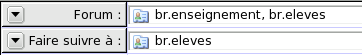
\includegraphics[width=0.45\textwidth]{images/cross_post_TB}
     & 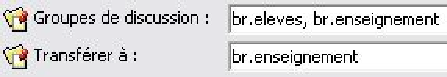
\includegraphics[width=0.45\textwidth]{images/cross_post_OE} \\
Thunderbird & Outlook Express
\end{tabular}


C'est bien plus simple que d'envoyer successivement ton message sur tous les \emph{newsgroups}, et la centralisation des réponses permet de conserver
un peu de clarté sur les \emph{newsgroups}, tout en te facilitant la vie. Que des avantages donc!


\subsubsection{Autres newsgroups}
Le site \urllink{polytechnique.org} dispose de son propre service de \emph{newsgroups}. Il sont
accessibles à tous les polytechniciens, qu'ils soient actuellement sur le campus ou membres de
promos précédentes. Pour plus d'informations, consulte \server{www.polytechnique.org}.

Il est aussi possible d'accéder à certains \emph{newsgroups} extérieurs à l'école via \server{polynews}. Ce serveur de la DSI est synchronisé avec
l'extérieur. Si tu cherches un \emph{newsgroup} qui ne s'y trouve pas, n'hésite pas à demander aux newsmestres.